\documentclass{math}

\usepackage{pgfplots}
\usepackage{tikz}

\geometry{letterpaper, margin=0.5in}
\pgfplotsset{compat=1.13}

\title{Differential Equations: Homework 8}
\author{Alvin Lin}
\date{January 2018 - May 2018}

\begin{document}

\maketitle
\clearpage

\section*{Section 4.6}

\subsubsection*{Exercise 1}
Find a general solution to the differential equation using the method of
variation of parameters.
\begin{align*}
  y''+4y &= \tan(2t) \\
  r^2+4 &= 0 \\
  r &= 0\pm2i \quad \alpha = 0 \quad \beta = 2 \\
  y_h &= c_1\cos(2t)+c_2\sin(2t) \\
  y_1 &= \cos(2t) \quad y_2 = \sin(2t) \\
  y_p &= v_1y_1+v_2y_2 \\
  W[y_1,y_2] &= \begin{vmatrix}
    \cos(2t) & \sin(2t) \\
    -2\sin(2t) & 2\cos(2t)
  \end{vmatrix} = 2\cos^2(2t)+2\sin^2(2t) = 2 \\
  v_1 &= -\int\frac{\tan(2t)\sin(2t)}{2}\diff{t} \\
  &= -\frac{1}{2}\int\frac{1-\cos^2(2t)}{\cos(2t)}\diff{t} \\
  &= -\frac{1}{2}\int\sec(2t)-\cos(2t)\diff{t} \\
  &= -\frac{1}{2}\bigg(\frac{\ln|\sec(2t)+\tan(2t)|-\sin(2t)}{2}\bigg) \\
  v_2 &= -\int\frac{\tan(2t)\cos(2t)}{2}\diff{t} \\
  &= -\frac{1}{4}\cos(2t) \\
  y_p &= \frac{-\ln|\sec(2t)+\tan(2t)|\cos(2t)-\sin(2t)\cos(2t)}{4}-
    \frac{\cos(2t)\sin(2t)}{4} \\
  y &= c_1\cos(2t)+c_2\sin(2t)-\frac{\ln|\sec(2t)+\tan(2t)|\cos(2t)}{4}
\end{align*}

\subsubsection*{Exercise 2}
Find a general solution to the differential equation using the method of
variation of parameters.
\begin{align*}
  y''+y &= \sec(t) \\
  r^2+1 &= 0 \\
  r &= 0\pm i \quad \alpha = 0 \quad \beta = 1 \\
  y_h &= c_1\cos(t)+c_2\sin(t) \\
  y_1 &= \cos(t) \quad y_2 = \sin(t) \\
  y_p &= v_1y_1+v_2y_2 \\
  W[y_1,y_2] &= \begin{vmatrix}
    \cos(t) & \sin(t) \\
    -\sin(t) & \cos(t)
  \end{vmatrix} = \cos^2(t)+\sin^2(t) = 1 \\
  v_1 &= -\int\frac{\sec(t)\sin(t)}{1}\diff{t} = -\ln|\sec(t)| \\
  v_2 &= \int\frac{\sec(t)\cos(t)}{1}\diff{t} = t \\
  y_p &= -\ln|\sec(t)|\cos(t)+t\sin(t) \\
  y &= c_1\cos(t)+c_2\sin(t)-\ln|\sec(t)|\cos(t)+t\sin(t)
\end{align*}

\subsubsection*{Exercise 4}
Find a general solution for the differential equation using the method of
variation of parameters.
\begin{align*}
  y''+2y'+y &= \e^{-t} \\
  r^2+2r+1 &= (r+1)^2 = 0 \\
  r &= -1 \\
  y_h &= c_1\e^{-t}+c_2t\e^{-t} \\
  y_1 &= \e^{-t} \quad y_2 = t\e^{-t} \\
  y_p &= v_1y_1+v_2y_2 \\
  W[y_1,y_2] &= \begin{vmatrix}
    \e^{-t} & t\e^{-t} \\
    -\e^{-t} & -t\e^{-t}+\e^{-t}
  \end{vmatrix} = \e^{-2t} \\
  v_1 &= -\int\frac{\e^{-2t}}{t\e^{-2t}}\diff{t} = -\frac{t^2}{2} \\
  v_2 &= \int\frac{\e^{-2t}}{\e^{-2t}}\diff{t} = t \\
  y_p &= -\frac{t^2\e^{-t}}{2}+t^2\e^{-t} \\
  y &= c_1\e^{-t}+c_2t\e^{-t}+\frac{t^2\e^{-t}}{2}
\end{align*}

\subsubsection*{Exercise 5}
Find a general solution for the differential equation using the method of
variation of parameters.
\begin{align*}
  y''(\theta)+16y(\theta) &= \sec(4\theta) \\
  r^2+16 &= 0 \\
  r &= 0\pm4i \quad \alpha = 0 \quad \beta = 4 \\
  y_h &= c_1\cos(4\theta)+c_2\sin(4\theta) \\
  y_1 &= \cos(4\theta) \quad y_2 = \sin(4\theta) \\
  y_p &= v_1y_1+v_2y_2 \\
  W[y_1,y_2] &= \begin{vmatrix}
    \cos(4\theta) & \sin(4\theta) \\
    -4\sin(4\theta) & 4\cos(4\theta)
  \end{vmatrix} = 4\cos^2(4\theta)+4\sin^2(4\theta) = 4 \\
  v_1 &= -\int\frac{\sec(4\theta)\sin(4\theta)}{4}\diff\theta =
    -\frac{\ln|\sec\theta|}{16} \\
  v_2 &= \int\frac{\sec(4\theta)\cos(4\theta)}{4}\diff\theta =
    \frac{\theta}{4} \\
  y_p &= \frac{-\ln|\sec\theta|\cos(4\theta)}{16}+
    \frac{\theta\sin(4\theta)}{4} \\
  y &= c_1\cos(4\theta)+c_2\sin(4\theta)+
    \frac{\theta\sin(4\theta)}{4}-\frac{\ln|\sec\theta|\cos(4\theta)}{16} \\
\end{align*}

\subsubsection*{Exercise 7}
Find a general solution to the differential equation using the method of
variation of parameters.
\begin{align*}
  y''+4t'+4y &= \e^{-2t}\ln(t) \\
  r^2+4t+4 &= (r+2)^2 = 0 \\
  r &= -2 \\
  y_h &= c_1\e^{-2t}+c_2t\e^{-2t} \\
  y_1 &= \e^{-2t} \quad y_2 = t\e^{-2t} \\
  y_p &= v_1y_1+v_2y_2 \\
  W[y_1,y_2] &= \begin{vmatrix}
    \e^{-2t} & t\e^{-2t} \\
    -2\e^{-2t} & -2t\e^{-2t}+\e^{-2t}
  \end{vmatrix} = \e^{-4t} \\
  v_1 &= -\int\frac{\e^{-2t}\ln(t)t\e^{-2t}}{\e^{-4t}}\diff{t} =
    -\int t\ln(t)\diff{t} = \frac{t^2}{4}-\frac{t^2\ln(t)}{2} \\
  v_2 &= \int\frac{\e^{-2t}\ln(t)\e^{-2t}}{\e^{-4t}}\diff{t} =
    \int\ln(t)\diff{t} = t\ln(t)-t \\
  y_p &= \frac{t^2\e^{-2t}}{4}-\frac{t^2\ln(t)\e^{-2t}}{2}+
    t^2\ln(t)\e^{-2t}-t^2\e^{-2t} \\
  &= \frac{t^2\ln(t)\e^{-2t}}{2}-\frac{3t^2\e^{-2t}}{4} \\
  y &= c_1\e^{-2t}+c_2t\e^{-2t}+
    \frac{t^2\ln(t)\e^{-2t}}{2}-\frac{3t^2\e^{-2t}}{4}
\end{align*}

\subsubsection*{Exercise 11}
Find a general solution to the differential equation.
\begin{align*}
  y''+y &= \tan(t)+\e^{3t}-1 \\
  r^2+1 &= 0 \\
  r &= 0\pm i \quad \alpha = 0 \quad \beta = 1 \\
  y_h &= c_1\cos(t)+c_2\sin(t) \\
  y_1 &= \cos(t) \quad y_2 = \sin(t) \\
  y_p &= v_1y_1+v_2y_2 \\
  W[y_1,y_2] &= \begin{vmatrix}
    \cos(t) & \sin(t) \\
    -\sin(t) & \cos(t)
  \end{vmatrix} = \cos^2(t)+\sin^2(t) = 1 \\
  v_1 &= -\int(\tan(t)+\e^{3t}-1)\sin(t)\diff{t} =
    \int\tan(t)\sin(t)-\e^{3t}\sin(t)+\sin(t)\diff{t} \\
  &= \sin(t)-\ln|\sec(t)+\tan(t)|-\frac{\e^{3t}(\cos(t)-3\sin(t))}{10}-
    \cos(t) \\
  v_2 &= \int(\tan(t)+\e^{3t}-1)\cos(t)\diff{t} =
    \int\sin(t)+\e^{3t}\sin(t)-\cos(t) \\
  &= -\cos(t)+\frac{\e^{3t}(\sin(t)+3\cos(t))}{10}-\sin(t) \\
  y_p &= \frac{\e^{3t}}{10}-\ln|\sec(t)+\tan(t)|\cos(t)-1 \\
  y &= c_1\cos(t)+c_2\sin(t)+\frac{\e^{3t}}{10}-\ln|\sec(t)+\tan(t)|\cos(t)-1
\end{align*}

\section*{4.9}

\subsubsection*{Exercise 1}
A 2-kg mass is attached to a spring with stiffness \( k = 50\frac{N}{m} \). The
mass is displaced \( \frac{1}{4}m \) to the left of the equilibrium point and
given a velocity of \( 1\frac{m}{sec} \) to the left. Neglecting damping, find
the equation of motion of the mass along with the amplitude, period, and
frequency. How long after release does the mass pass through the equilibrium
position?
\begin{align*}
  2y''+50y &= 0 \\
  y(0) &= -\frac{1}{4} \quad y'(0) = -1 \\
  2r^2+50 &= 0 \quad r = 0\pm5i \quad \alpha = 0 \quad \beta = 5 \\
  y(t) &= c_1\cos(5t)+c_2\sin(5t) \\
  y'(t) &= -5c_1\sin(5t)+5c_2\cos(5t) \\
  y(0) &= -\frac{1}{4} = c_1 \\
  y'(0) &= -1 = 5c_2 \quad c_2 = -\frac{1}{5} \\
  y(t) &= -\frac{1}{4}\cos(5t)-\frac{1}{5}\sin(5t)
\end{align*}
\begin{align*}
  A &= \sqrt{\bigg(\frac{1}{4}\bigg)^2+\bigg(\frac{1}{5}\bigg)^2} =
    \sqrt{\frac{41}{400}} \\
  T &= \frac{2\pi}{\omega} = \frac{2\pi}{5} \\
  f &= \frac{\omega}{2\pi} = \frac{5}{2\pi} \\
  \phi &= \arctan\bigg(\frac{c_1}{c_2}\bigg) = \arctan\bigg(\frac{5}{4}\bigg) \\
  y(t) &= \frac{\sqrt{41}}{20}\sin\bigg(5t+
    \arctan\bigg(\frac{5}{4}\bigg)\bigg) = 0 \\
  \sin\bigg(5t+\arctan\bigg(\frac{5}{4}\bigg)\bigg) &= 0 \\
  5t+\arctan\bigg(\frac{5}{4}\bigg) &= \pi \\
  t &= \frac{\pi-\arctan(\frac{5}{4})}{5}
\end{align*}

\subsubsection*{Exercise 3}
The motion of a mass-spring system with damping is governed by
\[ y''(t)+by'(t)+16y(t) = 0 \quad y(0) = 1 \quad y'(0) = 0 \]
Find the equation of motion and sketch its graph for \( b = 0,6,8,10 \). \\
\begin{align*}
  b &= 0 \\
  y''(t)+16y(t) &= 0 \\
  r^2+16 &= 0 \quad r = 0\pm4i \quad \alpha = 0 \quad \beta = 4 \\
  y(t) &= c_1\cos(4t)+c_2\sin(4t) \\
  y'(t) &= -4c_1\sin(4t)+4c_2\cos(4t) \\
  y(0) &= 1 = c_1 \\
  y'(0) &= 0 = 4c_2 \quad c_2 = 0 \\
  y(t) &= \cos(4t) \\
\end{align*}
\begin{align*}
  b &= 6 \\
  y''(t)+6y'(t)+16y(t) &= 0 \\
  r^2+6r+16 &= 0 \\
  r &= \frac{-6\pm\sqrt{36-4(1)(16)}}{2} \\
  &= -3\pm\sqrt{7}i \quad \alpha = -3 \quad \beta = \sqrt{7} \\
  y(t) &= \e^{-3t}(c_1\cos(\sqrt{7}t)+c_2\sin(\sqrt{7}t)) \\
  y'(t) &= \e^{-3t}(-\sqrt{7}c_1\sin(\sqrt{7}t)+\sqrt{7}c_2\cos(\sqrt{7}t))+
    -3\e^{-3t}(c_1\cos(\sqrt{7}t)+c_2\sin(\sqrt{7}t)) \\
  y(0) &= 1 = c_1 \\
  y'(0) &= 0 = \sqrt{7}c_2-3c_1 \quad c_2 = \frac{3}{\sqrt{7}} \\
  y(t) &= \e^{-3t}(\cos(\sqrt{7}t)+\frac{3}{\sqrt{7}}\sin(\sqrt{7}t))
\end{align*}
\begin{align*}
  b &= 8 \\
  y''(t)+8y'(t)+16y(t) &= 0 \\
  r^2+8r+16 &= (r+4)^2 = 0 \\
  r &= -4 \\
  y(t) &= c_1\e^{-4t}+c_2t\e^{-4t} \\
  y'(t) &= -4c_1\e^{-4t}-4c_2t\e^{-4t}+c_2\e^{-4t} \\
  y(0) &= 1 = c_1 \\
  y'(0) &= 0 = -4c_1+c_2 \quad c_2 = 4 \\
  y(t) &= \e^{-4t}+4t\e^{-4t}
\end{align*}
\begin{align*}
  b &= 10 \\
  y''(t)+10y'(t)+16y(t) &= 0 \\
  r^2+10r+16 &= (r+8)(r+2) = 0 \\
  r &= -8 \quad r = -2 \\
  y(t) &= c_1\e^{-8t}+c_2\e^{-2t} \\
  y'(t) &= -8c_1\e^{-8t}-2c_2\e^{-2t} \\
  y(0) &= 1 = c_1+c_2 \\
  y'(0) &= 0 = -8c_1-2c_2 \\
  c_1 &= -\frac{1}{3} \quad c_2 = \frac{4}{3} \\
  y(t) &= -\frac{1}{3}\e^{-8t}+\frac{4}{3}\e^{-2t}
\end{align*}
\begin{center}
  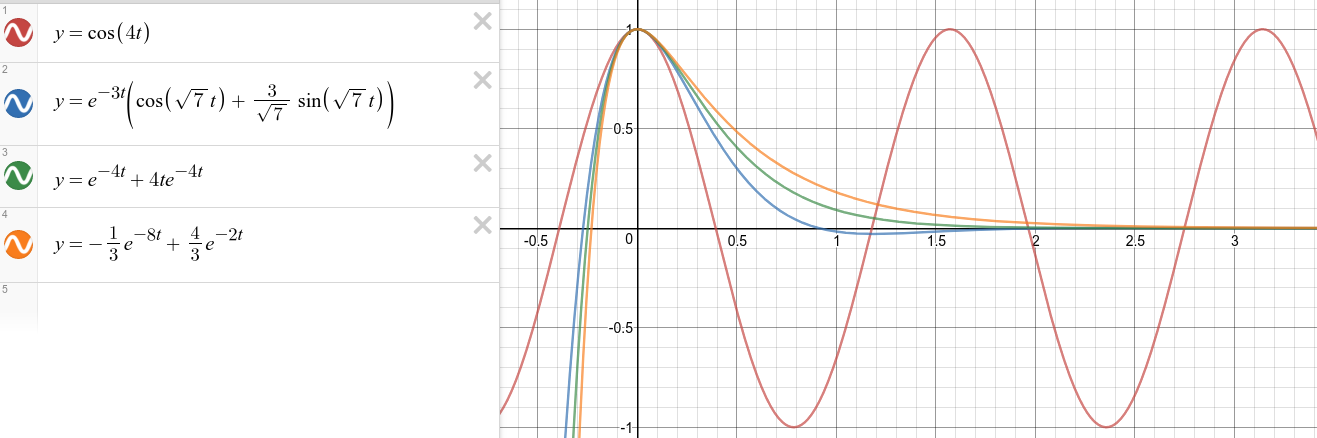
\includegraphics[width=20cm]{assets/hw_08_07.png}
\end{center}

\subsubsection*{Exercise 7}
A \( \frac{1}{8}kg \) mass is attached to a spring with stiffness
\( 16\frac{N}{m} \). The damping constant for the system is
\( 2\frac{N\cdot sec}{m} \). If the mass is moved \( \frac{3}{4}m \) to the left
of equilibrium and given an initial leftward velocity of \( 2\frac{m}{sec} \),
determine the equation of motion of the mass and give its damping factor,
quasiperiod, and quasifrequency.
\begin{align*}
  \frac{1}{8}y''+2y'+16y &= 0 \quad y(0) = -\frac{3}{4} \quad y'(0) = -2 \\
  \frac{1}{8}r^2+2r+16 &= 0 \\
  r^2+16r+128 &= 0 \\
  r &= \frac{-16\pm\sqrt{16^2-4(1)(128)}}{2} = -8\pm8i \quad \alpha = -8 \quad
    \beta = 8 \\
  y(t) &= \e^{-8t}(c_1\cos(8t)+c_2\sin(8t)) \\
  y'(t) &= \e^{-8t}(-8c_1\sin(8t)+8c_2\cos(8t))-
    8\e^{-8t}(c_1\cos(8t)+c_2\sin(8t)) \\
  y(0) &= -\frac{3}{4} = c_1 \\
  y'(0) &= -2 = 8c_2-8c_1 \quad c_2 = -1 \\
  y(t) &= \e^{-8t}(-\frac{3}{4}\cos(8t)-\sin(8t)) \\
  &= -\frac{3\e^{-8t}}{4}\cos(8t)-\e^{-8t}\sin(8t) \\
  A &= \sqrt{c_{1'}^2+c_{2'}^2} = \sqrt{\frac{25}{16}\e^{-16t}} =
    \frac{5}{4}\e^{-8t} \\
  \omega &= \sqrt{\frac{k}{m}} = \sqrt{\frac{16}{0.125}} \\
  T &= \frac{2\pi}{\beta} = \frac{2\pi}{8} = \frac{\pi}{4} \\
  f &= \frac{\beta}{2\pi} = \frac{4}{\pi}
\end{align*}

\begin{center}
  If you have any questions, comments, or concerns, please contact me at
  alvin@omgimanerd.tech
\end{center}

\end{document}
